To verify proposed approaches, the mobile application as proof-of-concept was implemented. For verification was chosen especially process instance visualisation.

The given application offers:
\begin{enumerate}
\item Process instance visualisation with simulated data
\item Concept of dashboard
\end{enumerate}

Frstly the used technologies are introduced. Then the brief architecture of mobile application and implementation itself are explained. In the end, the issues with implementation are described. 
% ---------------------------------------------------------------------------------
\section{.NET Platform}

For implementation is used .NET platform and programming language C\#. The .NET is free, open-source and cross-platform framework for building many different types of applications~\cite{what-is-dotnet}. There is a lot of frameworks within platform, such as WPF for building native desktop applications for Windows or ASP .NET framework for building websites and server-side applications. Also there is cross-platform Xamarin framework for building mobile applications. These all frameworks were used to implement proof-of-concept. 
% ---------------------------------------------------------------------------------
\subsection{.NET Standard}
\begin{figure}[ht!]
\centering
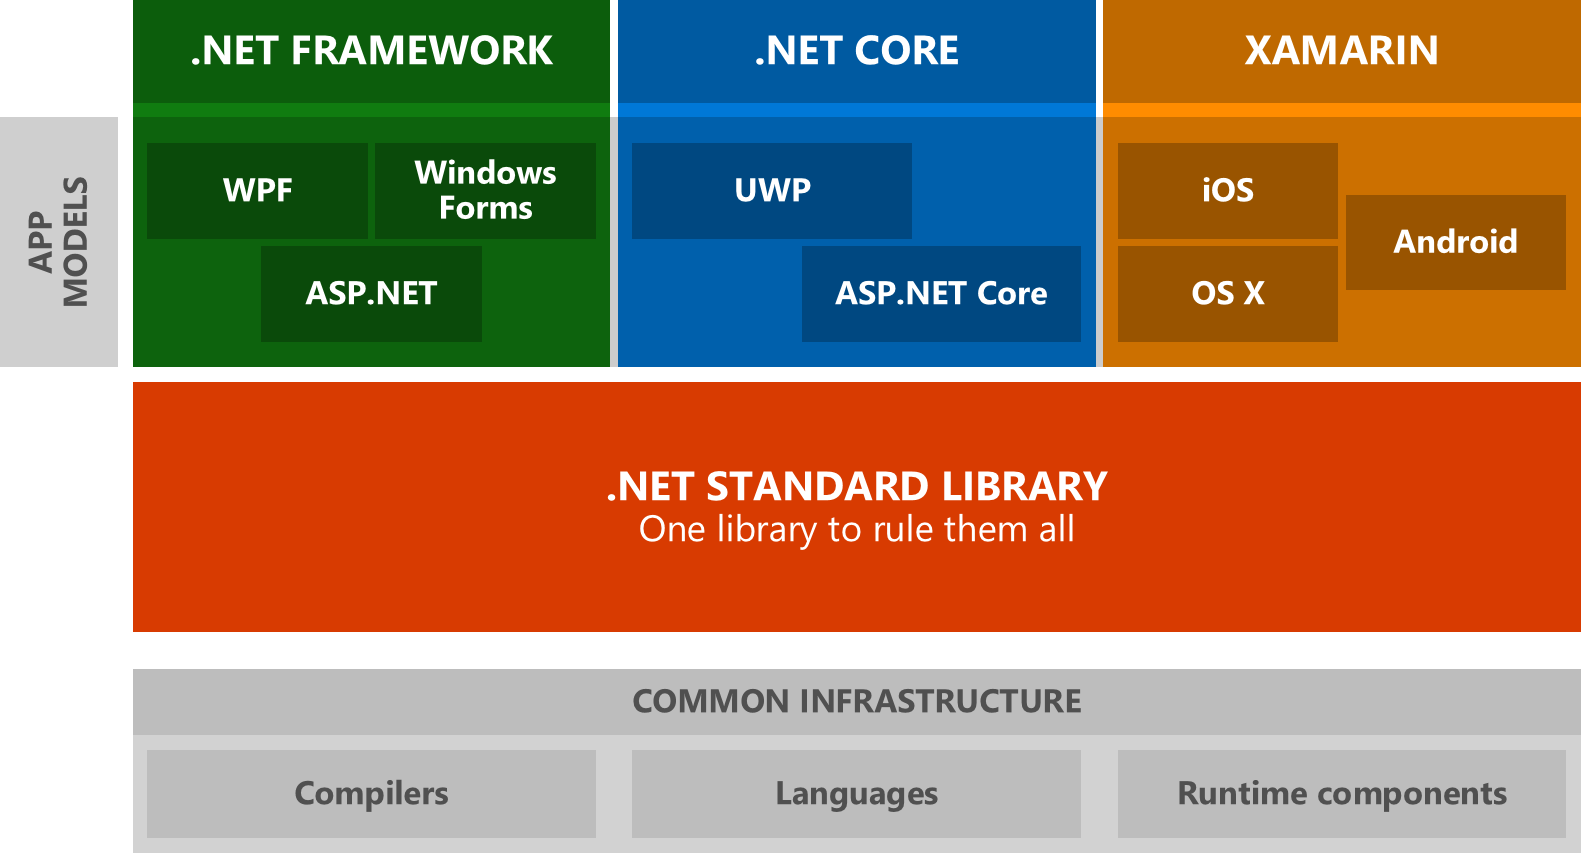
\includegraphics[width=12cm,keepaspectratio]{img/dotnet-overview}
\caption{The .NET platform overview \cite{introducing-dotnet-standard}}
\label{fig:dotnet-overview}
\end{figure}

Earlier years within .NET platform was problem with many different implementations of .NET itself. There was the ``original'' (full) .NET. Then a newer, open-source and cross-platform version .NET Core and third was Xamarin. Each platform have different base libraries and if developers wanted to share code between these platforms, there was a lot of work to do. 

The new approach was introduced~\cite{introducing-dotnet-standard}. The .NET Standard is the unified platform which defines set of APIs that each .NET subset platform must implement. This allows to developers easily share code and write libraries that can be used anywhere. The great graphical summarization is shown at \cref{fig:dotnet-overview}. Actual version is .NET Standard 2.0. The newer version 2.1 will be introduced within Q2 2018. 
% ---------------------------------------------------------------------------------
\subsection{.NET Core}
The .NET Core is open-source, cross-platform version of .NET Framework. It is new and highly frequently updated framework which becomes very popular. It has many ``ports'' of frameworks from full .NET such as ASP .NET or Entity Framework -- an Object-Relationship-Mapping tool for databases. 
% ---------------------------------------------------------------------------------
\section{Xamarin}
Xamarin is platform for developing native mobile applications in cross-platform way. Developers use C\# language and .NET Standard to implement mobile application. When the application is being build, the code is compiled to native platform code. 

Following summarization is taken from~\cite{xamarin-understand-platform}:
\begin{itemize}
\item On iOS, C\# is ahead-of-time (AOT) compiled to ARM assembly language. The .NET framework is included, with unused classes being stripped out during linking to reduce the application size. Apple does not allow runtime code generation on iOS, so some language features are not available.
\item On Android, C\# is compiled to IL and packaged with MonoVM. Unused classes in the framework are stripped out during linking. The application runs side-by-side with Android runtime.
\item Windows and UWP use directly C\# and included .NET. 
\end{itemize}

Within Xamarin there are two main approaches how to build applications (see \cref{fig:xamarin-native-vs-forms}). First one is commonly called ``Xamarin Native'' or ``Xamarin.*'' where * is targeted platform. With this approach, the code for business logic is written independently from target platform, but user interface for each platform is implemented separately with native approaches (e.g. for Android developer uses XML based declarations).

\begin{figure}[ht!]
\centering
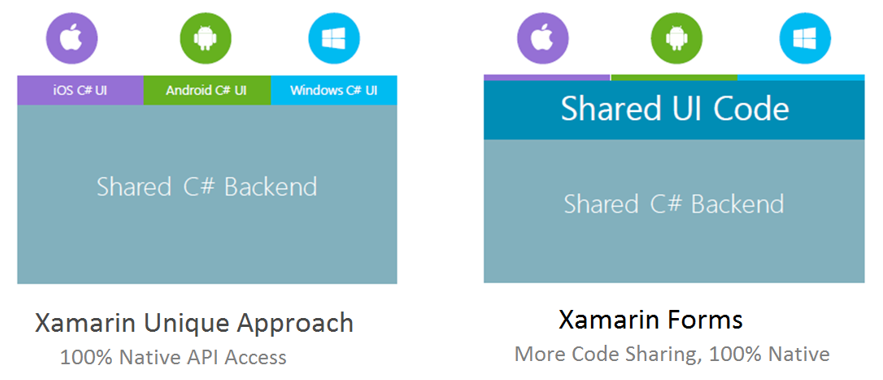
\includegraphics[width=12cm,keepaspectratio]{img/xamarin-vs-xamarin-forms}
\caption{The Xamarin.* vs. Xamarin.Forms \cite{xamarin-native-forms}}
\label{fig:xamarin-native-vs-forms}
\end{figure}

\begin{figure}[ht!]
\centering
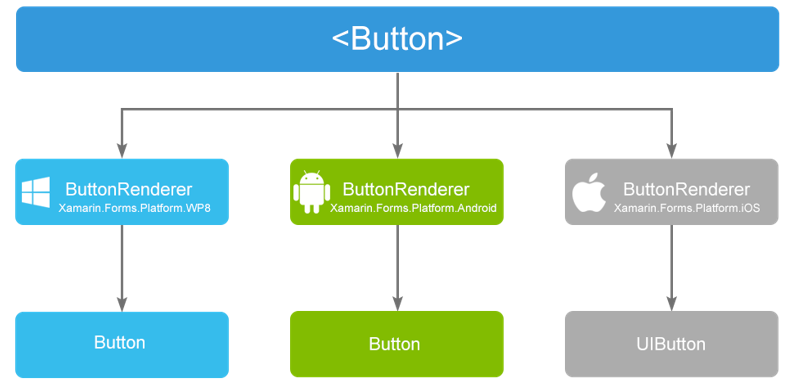
\includegraphics[width=10cm,keepaspectratio]{img/xamarin-forms-ui-render}
\caption{The Xamarin.Forms control renderer \cite{xamarin-native-forms}}
\label{fig:xamarin-ui-renderer}
\end{figure}

Second one is called Xamarin.Forms, which is build on top of first one and allows to define user interfaces in cross-platform way. Developers use XAML, the declaration language similar to XML to define user interface. When application is being build, defined controls are transformed to native controls. This transformation is done through concept called ``Control renderer''. Within shared library, an interface for control is defined. On each platform is implemented renderer which transforms given control to native one. An example is shown at \cref{fig:xamarin-ui-renderer}.
% ---------------------------------------------------------------------------------
\section{Another Used Technologies}
The implementation is divided to two parts. First one is mobile application and second one is server-side, the concept of \textit{Data Aggregation Service}. 

For server-side implementation was chosen ASP .NET Core -- a newer version of ASP .NET, framework for creating server applications  (services, REST API, \dots) and websites.

Within ASP .NET Core a web application was created and library SignalR was chosen for real-time communication between clients and server.
% ---------------------------------------------------------------------------------
\subsection{SignalR}
\begin{figure}[ht!]
\centering
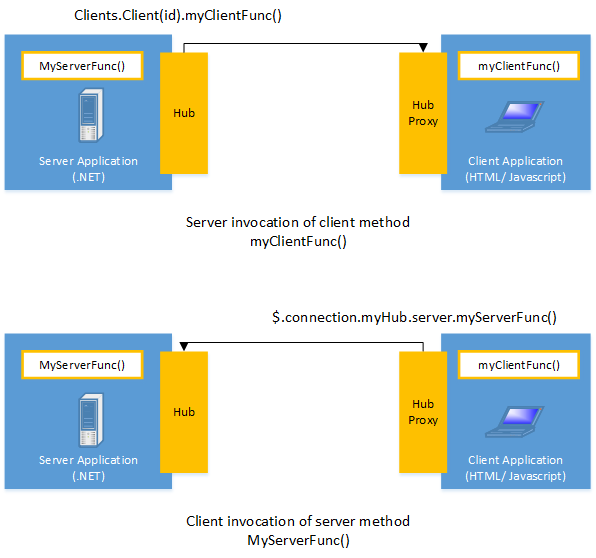
\includegraphics[width=8cm,keepaspectratio]{img/signal-r-overview}
\caption{How SignalR works \cite{signal-r-overview}}
\label{fig:signal-r-overview}
\end{figure}
According to~\cite{signal-r-overview} SignalR is: ``a library for ASP .NET which offers adding real-time web functionality to applications. Real-time web functionality is the ability to have server code push content to connected clients instantly as it becomes available, rather than having the server wait for a client to request new data''. SignalR handles ``many things'' for developers automatically, such as connection management or choosing transporting types. SignalR firstly try to use WebSocket and if it fails, automatically fall back to older transports.

On the server, developer defines a \textit{Hub}. \textit{Hub} defines contract which clients will use and communicate through. On the client-side, developers creates \textit{Hub Proxy} -- connection to specific \textit{Hub}. The example how it works is shown at \cref{fig:signal-r-overview}.
% ---------------------------------------------------------------------------------
\section{Implementation Decisions}
For implementation were chosen a quite new and interesting technologies and combinations of them.
The .NET Standard is for now the only one right way how to create shared C\# back-end. Older approaches with \gls{pcl} are deprecated and Xamarin recommends to use .NET Standard. Although it is recommended and \gls{pcl} are deprecated, many problems occurred. More discussion about problems with implementation is in the end of this chapter.

For mobile-application was chosen Xamarin.Forms for this reasons:
\begin{itemize}
\item Author has many experiences with XAML from similar frameworks such as WPF or Universal Windows Platform.
\item Xamarin.Forms are more faster for developing with cross-platform way -- the user interface is written once.
\end{itemize}

Xamarin.Forms offers many prepared controls for use, but for creation of process instance visualisation a custom controls were created.  

A many different approaches were tried. First one was edit already existing controls, but it was found, that it is not suitable. Another approach was to find existing controls, which resulted to, that the requirements are too specific and required controls do not exists. Third option was to use some basic 2D engine for custom drawing and rendering. The third option seemed as best option to do, so it was chosen. 
% ---------------------------------------------------------------------------------
\subsection{SkiaSharp}
SkiaSharp library~\cite{skiasharp} provides a way how to quickly and easily do custom 2D drawing. It is used for process visualisation. Each \textit{transaction box} is custom control created with SkiaSharp's canvas -- a place-holder for custom drawings. Each \textit{transaction link} is also custom controls made with this library. 
% ---------------------------------------------------------------------------------
\subsection{Syncfusion Controls Library}
Syncfusion Controls Library~\cite{syncfusion} adds many new controls to Xamarin.Forms. The Dashboard uses this library for its various types of charts. 
% ---------------------------------------------------------------------------------
\subsection{Simulation Cases}
Main goal of proof-of-concept is to verify that proposed visualisation approach is usable. In real-world usage, many other systems and services must be developed. Also there is not any ``real-world'' data source. For this reason, the simulation approach was chosen. As base model is chosen Rent-A-Car company. From RAC model several simulation cases are preapred.
% ---------------------------------------------------------------------------------
\section{Implementation Details}
Only fundamental implementation decisions and circumstances are described. At the \cref{fig:impl-dependecies-graph} is shown ``high-level'' architecture of application:

\begin{figure}[ht!]
\centering
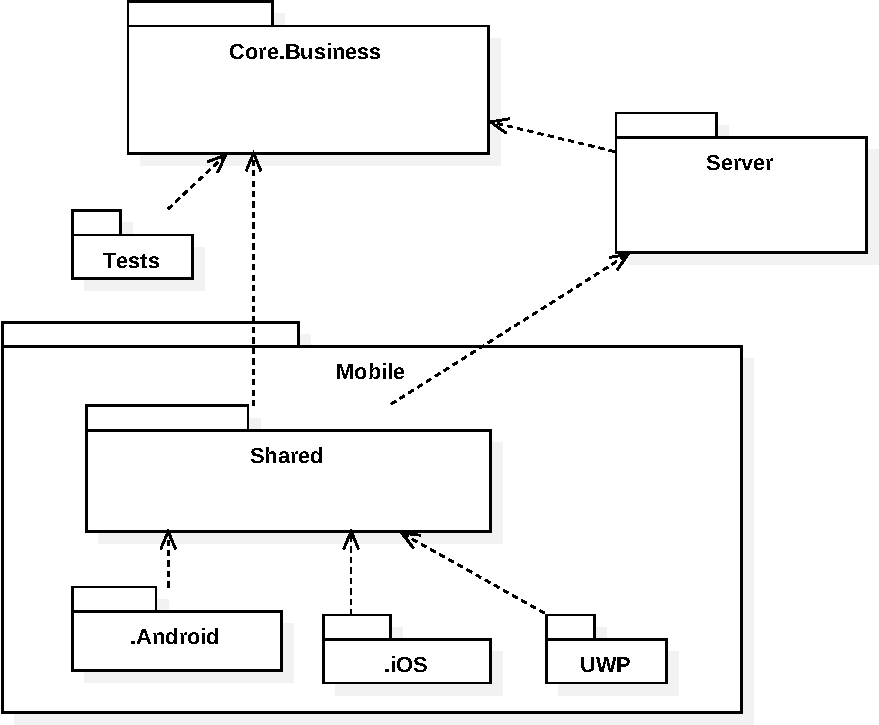
\includegraphics[width=10cm,keepaspectratio]{img/dependecies-graph}
\caption{The implementation packages}
\label{fig:impl-dependecies-graph}
\end{figure}

\begin{description}
\item[Core.Business] -- The \textit{Data Domain Model} is placed here, because mobile and server applications use it. Also classes for simulations and XML parsers are there.
\item[Server] -- The simple ASP .NET Core with SignalR application for serving a simulation data.
\item[Mobile.Shared] -- A shared part of Xamarin application. All business logic and user interface are implemented here.
\item[Mobile.Shared.Android] -- A Xamarin.Android project. There are Android specific implementations and initialization for Xamarin.Forms. Also all the graphic assets (logo, icons, \dots) are placed in this project.
\item[Mobile.Shared.iOS] -- A Xamarin.iOS project. Same purpose as Mobile.Shared.Android.
\item{Mobile.Shared.UWP} -- A Xamarin.UWP (Universal Windows Platform) project. Same purpose as Mobile.Shared.Android.
\item[Tests] -- Package contains several unit tests for Core.Business. 
\end{description}
% ---------------------------------------------------------------------------------
\subsection{The Dashboard}
As has been said, Dashboard uses several charts from Syncfusion library. Each chart is predefined and customized for better look. 
% ---------------------------------------------------------------------------------
\subsection{Simulation Cases}
Each simulation cases is defined as XML file. Because creating and writing testing data within XML is not so comfortable, the simple utility was implemented. The utility allows interactively define new simulation case.

Each simulation case has three parts:
\begin{itemize}
\item First part defines \textit{Actors} -- the instances of \textit{Actor Roles}.
\item Second part defines \textit{Process Instance} with \textit{Transaction Instances}.
\item Third part defines simulation \textit{chunks}. Each chunks store one or more \textit{Events}.
\end{itemize}

When simulation case runs, every ``simulation step'' new chunk is loaded and all events from chunk are returned to client. With this approach, it can simulate incoming data from real data source.

The utility allows to define chunks and events with interactive editor, where user can simply fill transaction id, event type, time creation and type of C-Act. An example of simulation case:

\begin{minted}[breaklines, breakaftersymbolpre= ]{xml}
<?xml version="1.0" encoding="utf-8"?>
<Simulation Name="Case02">
  <Actors>
    <Actor Id="1" ActorRoleId="1" FirstName="George" LastName="Lucas" />
    <Actor Id="2" ActorRoleId="2" FirstName="George" LastName="Lucas" />
    <Actor Id="3" ActorRoleId="3" FirstName="Bob" LastName="Freeman" />
    <Actor Id="4" ActorRoleId="4" FirstName="Alice" LastName="Freeman" />
  </Actors>
  <ProcessInstance Id="1" KindId="1" StartTime="01-02-2018 15:34:23" ExpectedEndTime="01-02-2018 15:34:23">
    <TransactionInstance Id="1" KindId="1" Identificator="T1" CompletionType="0" ProcessInstanceId="1" InitiatorId="0" ExecutorId="0" ParentId="0">
      <TransactionInstance Id="2" KindId="2" Identificator="T2" CompletionType="0" ProcessInstanceId="1" InitiatorId="0" ExecutorId="0" ParentId="1" />
    </TransactionInstance>
    <TransactionInstance Id="3" KindId="3" Identificator="T3" CompletionType="0" ProcessInstanceId="1" InitiatorId="0" ExecutorId="0" ParentId="0">
      <TransactionInstance Id="4" KindId="4" Identificator="T4" CompletionType="0" ProcessInstanceId="1" InitiatorId="0" ExecutorId="0" ParentId="3" />
      <TransactionInstance Id="5" KindId="5" Identificator="T5" CompletionType="0" ProcessInstanceId="1" InitiatorId="0" ExecutorId="0" ParentId="3" />
    </TransactionInstance>
  </ProcessInstance>
  <Chunks>
    <Chunk>
      <Event Type="0" TransactionId="1" TransactionKindId="1" RaisedById="1" Created="01-02-2018 09:00:00">
        <CompletionChanged Completion="Requested" />
      </Event>
    </Chunk>
    <Chunk>
      <Event Type="0" TransactionId="1" TransactionKindId="1"  RaisedById="4" Created="01-02-2018 09:01:00">
        <CompletionChanged Completion="Declined" />
      </Event>
    </Chunk>
    <Chunk>
      <Event Type="0" TransactionId="1" TransactionKindId="1"  RaisedById="1" Created="01-02-2018 09:01:10">
        <CompletionChanged Completion="Quitted" />
      </Event>
    </Chunk>
  </Chunks>
</Simulation>
\end{minted}
% ---------------------------------------------------------------------------------
\subsection{Process Visualisation}
The process instance visualisation is done as follows:
\begin{enumerate}
\item Simulation case is loaded through \mintinline{C}{SimulationProvider}.
\item Process instance from simulation case is passed to \mintinline{C}{GanttChartBuilder}. This class is responsible for creating \textit{Transaction Boxes} and \textit{Transaction links} controls and wiring them together.
\item Created controls are inserted to \mintinline{C}{RelativeLayout} control. This control allows to place controls relatively to another. 
\end{enumerate}

A note about the Transaction Box Control. It derives from \mintinline{C}{SKCanvasView}, which comes from SkiaSharp. The class provides method \mintinline{C}{OnPaintSurface} which is called every time when the graphics must be refreshed. An argument \mintinline{C}{SKPaintSurfaceEventArgs} provides \mintinline{C}{SKCanvas} which contains methods for basic 2D drawing. 
% ---------------------------------------------------------------------------------
\section{Application Testing}
The mobile application as a whole product were tested manually several times. Several people were familliared to  thesis problematic and tried to use the application. The main part of manual testing was done on process visulisation, where were main issues with usability. 

Based on this manual testing and response from testers, the whole concept of visualisaiton was several times modified. 
\begin{itemize}
\item Application force landscape orientation for process visualisation. The portrait orientation not useful.
\item The time-line size is bigger due to fact, that earlier version had too small font and it was barely readable.
\item As has been said in \cref{ch:proposed-approach}, first intent was to wire time-line and transaction boxes together. First implemented concept showed that due to smaller screen sizes, user must often scroll to get information -- it was unclear and unusable. The result is nearly two independent parts where each serves for another purpose. 
\end{itemize}
% ---------------------------------------------------------------------------------
\section{Implementation Issues and Consequences}
The implementation uses .NET Standard 2.0. This version is recommended for new Xamarin applications. But many used libraries, such as SkiaSharp (which is originally written as PCL) are ported to work within .NET Standard.

During implementation many issues occurred, especially with Xamarin and SignalR library.
% ---------------------------------------------------------------------------------
\subsection{Xamarin.Forms Issues}
As has been said there are two main approaches how to develop with Xamarin platform. For implementation was chosen Xamarin.Forms. During implementation many issues with compatibility, run-time errors and bugs occurred. 

Although Xamarin platform is not new and it is well used, there are still many issues, which make development very hard, sometimes nearly impossible. There are few common issues. For example:
\begin{itemize}
\item Sometimes shared code behaves differently on each platforms. For example, simple selecting item within ListView control (a list of items which is scrollable). On UWP platform, the ListView selected different item than the real one. 
\item Debugging application hangs with unknown errors.
\item Many issues with compiling XAML and ``fake'' error messages. 
\end{itemize}

Fortunately, this issues are addressed and they are in repairing process. These issues led to, that only Android platform is tested. UWP platform was during development omitted due to incompatibility with current version. The iOS platform was omitted at the beginning, because development for this platform requires device with macOS. 

In the end, result is that Xamarin.Native could be a better approach. Xamarin.Forms are really great for form-based applications, but if developers want something really specific, it is better to define user interfaces within each platform separately. 
% ---------------------------------------------------------------------------------
\subsection{SignalR Core Issues}
The SignalR for now is in the development process. Although it is supported with .NET Standard 2.0 during development was find out, that there are incompatibility issues between SignalR Core, .NET Standard 2.0 and Xamarin platform. Again this issue is reported and it will be repaired with version 2.1 which will come out in Q2 2018.

This issue led to two things:
\begin{enumerate}
\item The server-side and mobile clients are separated. On the mobile client, the fake embedded server is included -- simulation are loaded within mobile application itself and it behaves like server communication. 
\item The server side is implemented and tested through simple JavaScript client, which works as expected. 
\end{enumerate}
% ---------------------------------------------------------------------------------
\section{The Result}
The goal of implementation was successfully completed, despite the described issues. The process visualisation is implemented and proofed with prepared simulation cases. The mobile application is implemented as ``Mobile Service for Rent-A-Car  company''. Following figures show the result. 


\begin{figure}[ht!]
 \centering
 \subfloat{{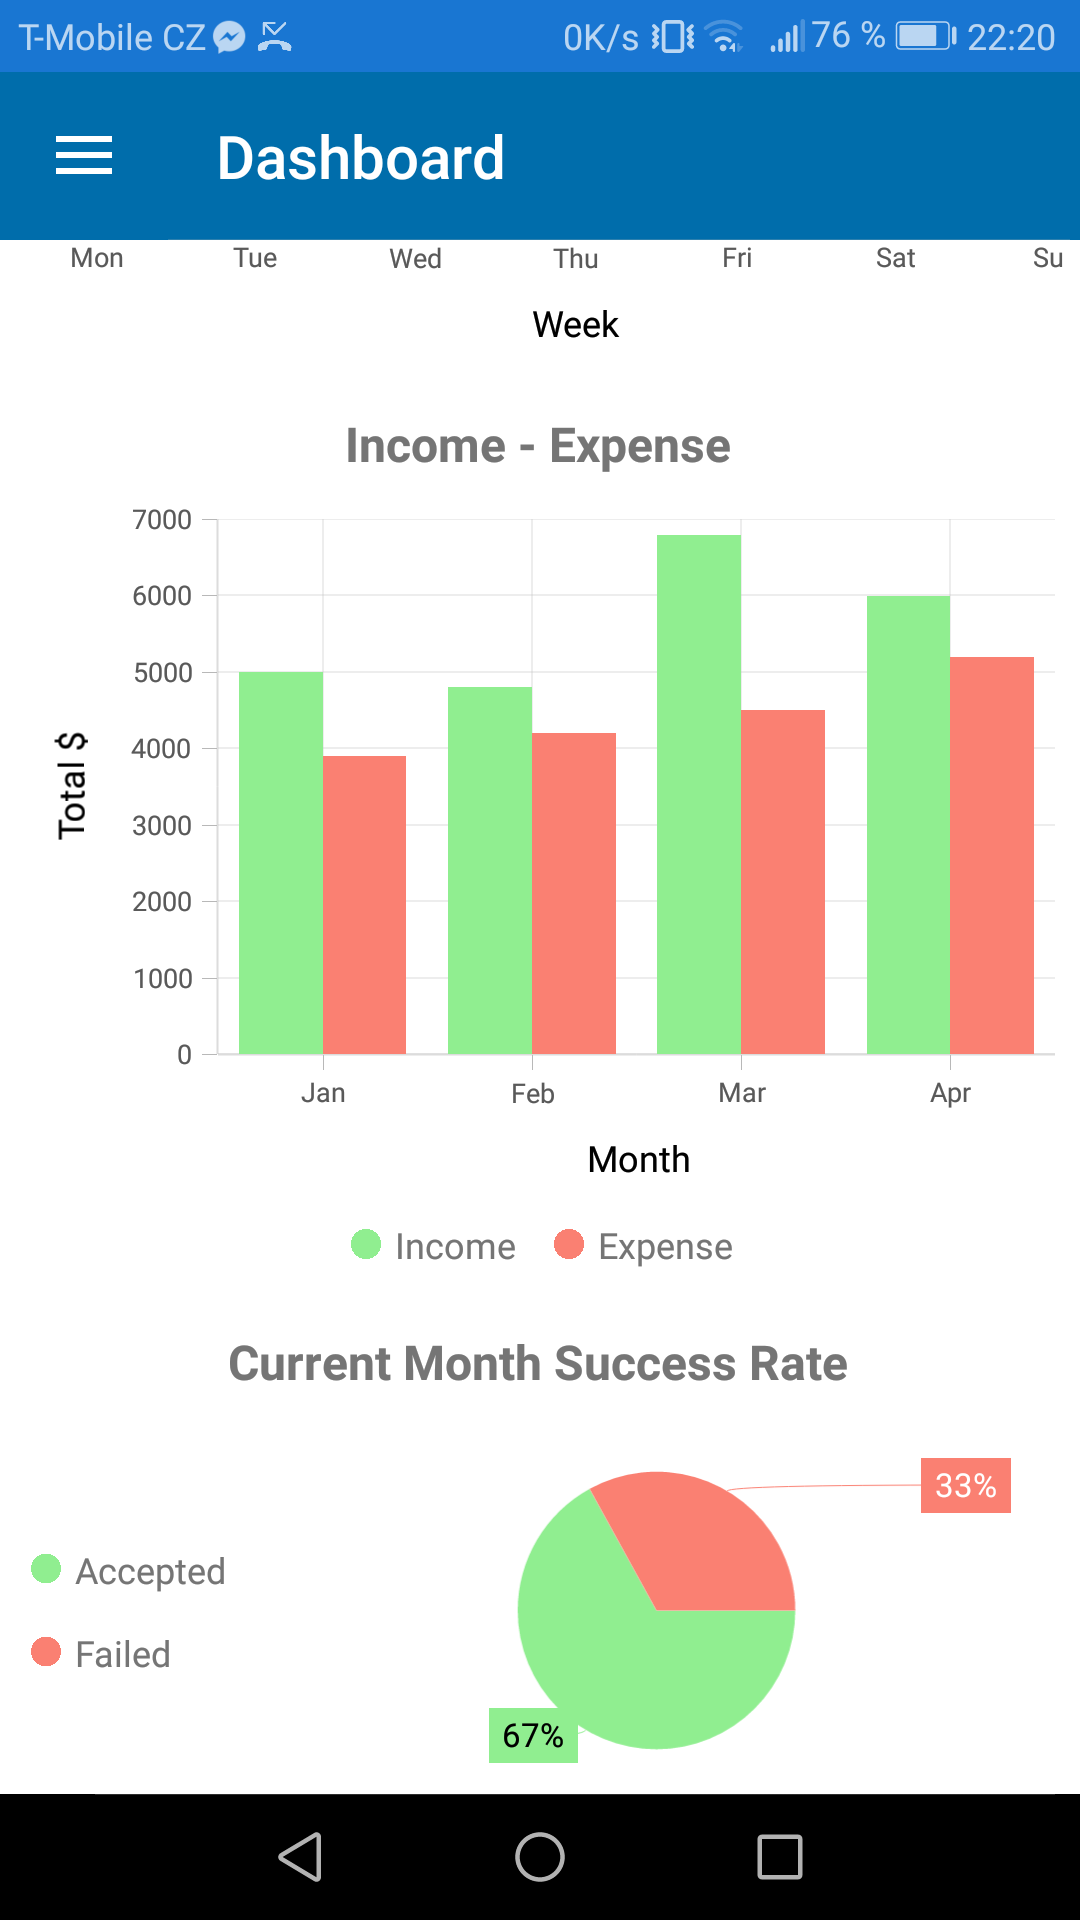
\includegraphics[width=6cm, keepaspectratio]{img/app-dashboard} }}%
 \qquad
 \subfloat{{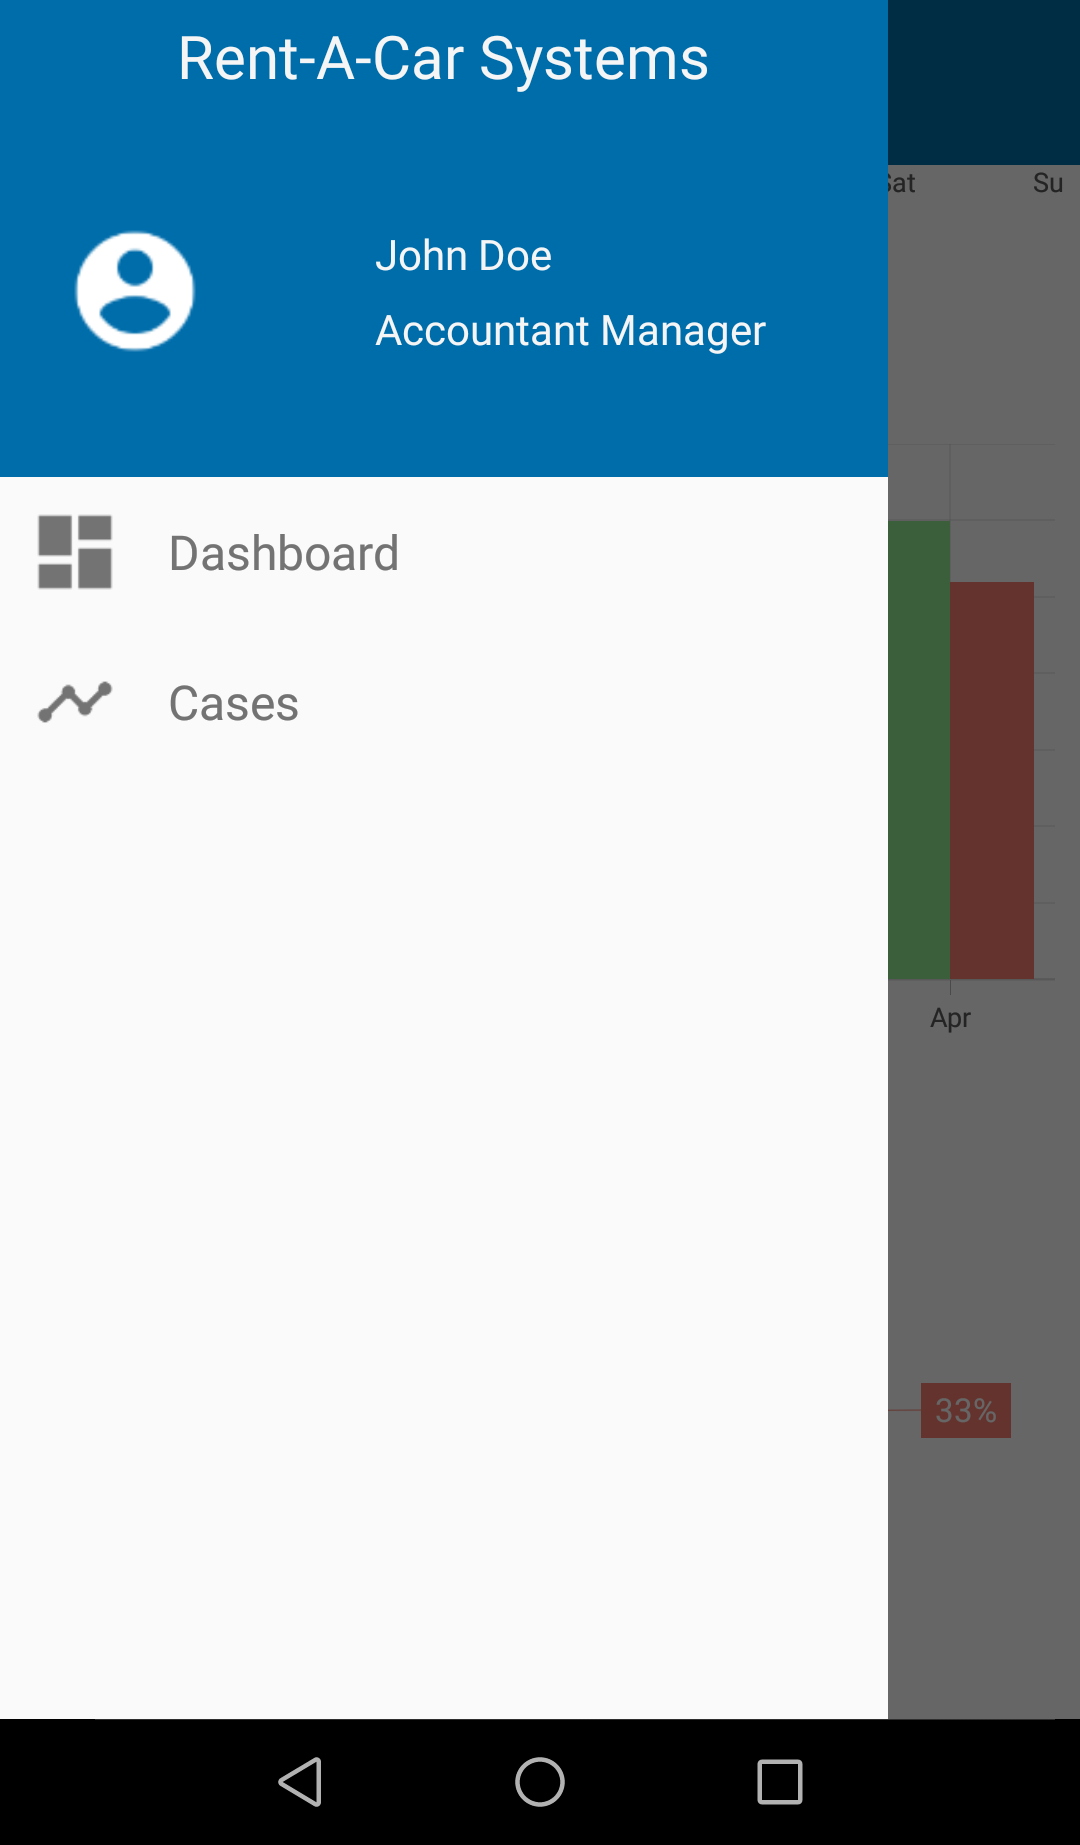
\includegraphics[width=6cm, keepaspectratio]{img/app-menu} }}%
 \caption{The Dashboard (on the left) and the menu (on the right)}%
 \label{fig:app-dashboard-menu}%
\end{figure}

\begin{figure}[ht!]
\centering
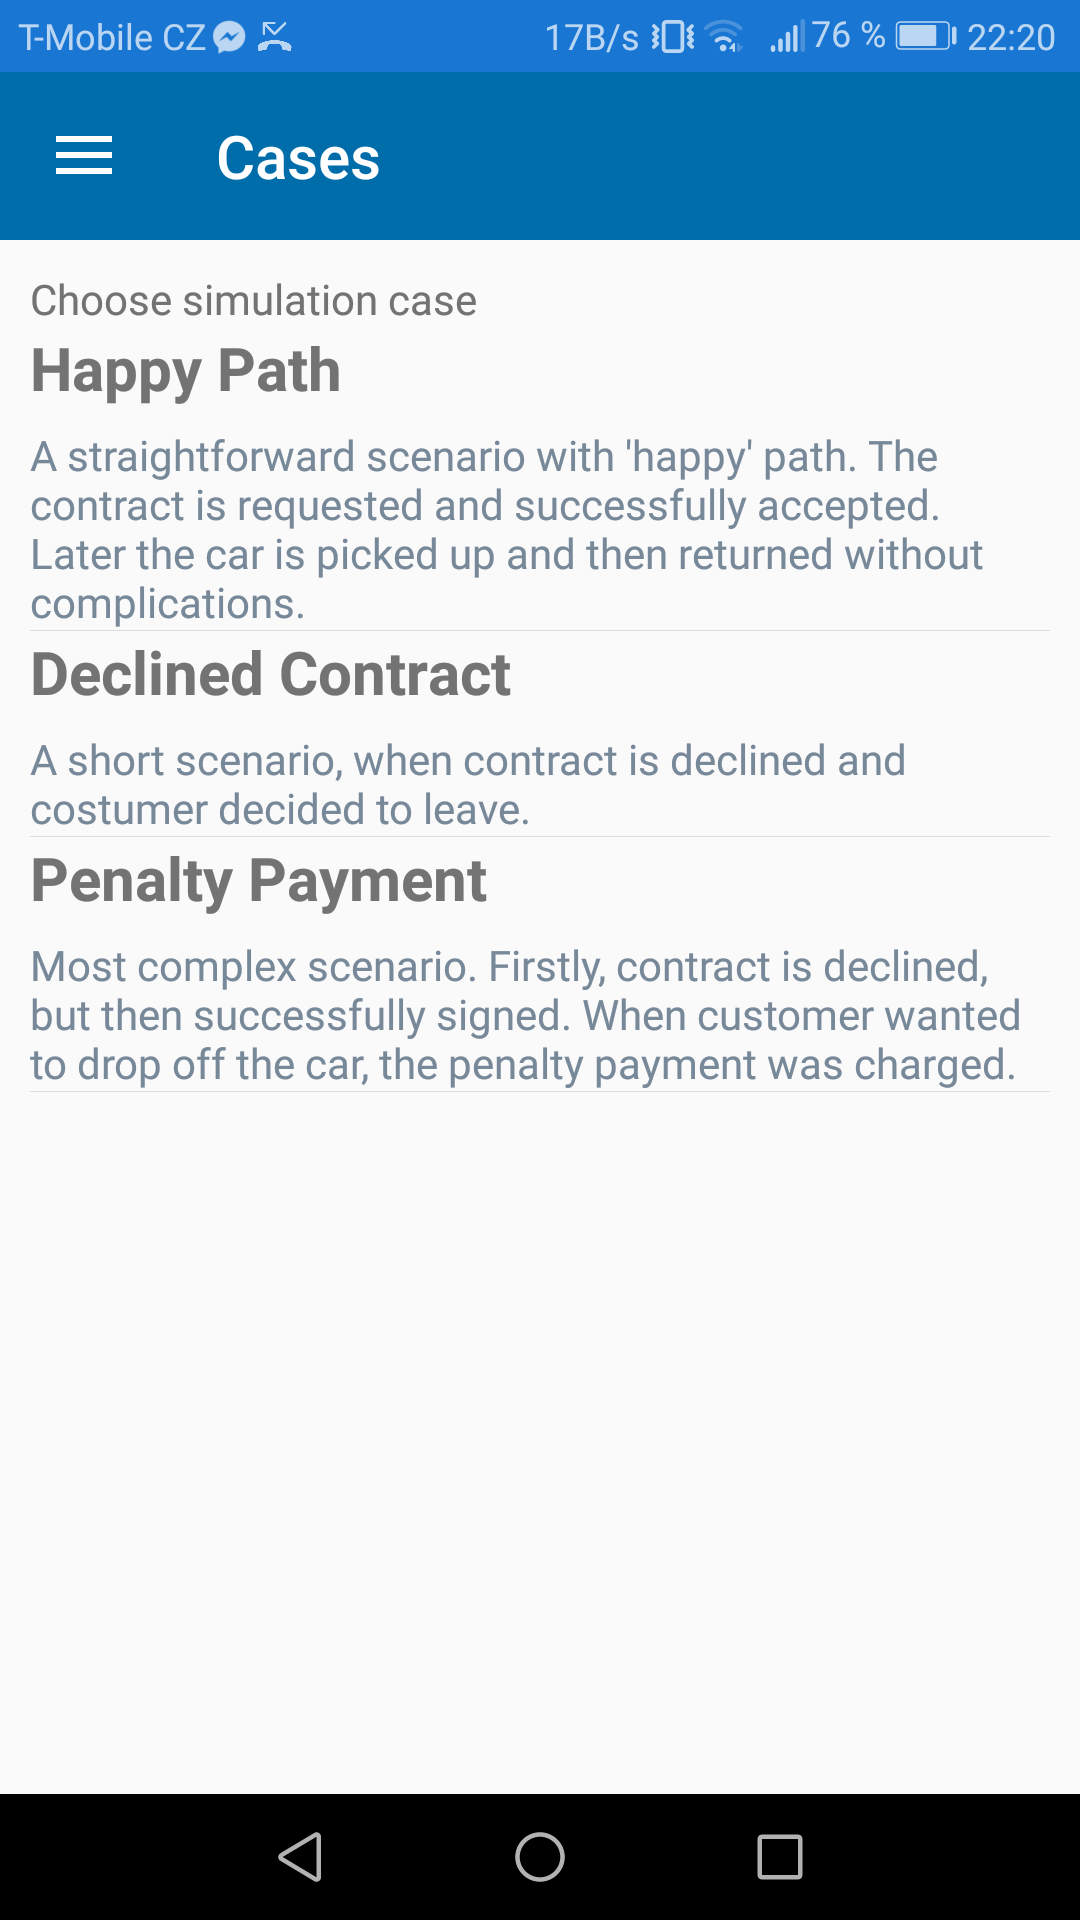
\includegraphics[width=6cm,keepaspectratio]{img/app-process-list}
\caption{The predefined simulation cases}
\label{fig:app-list}
\end{figure}

\begin{figure}[ht!]
\centering
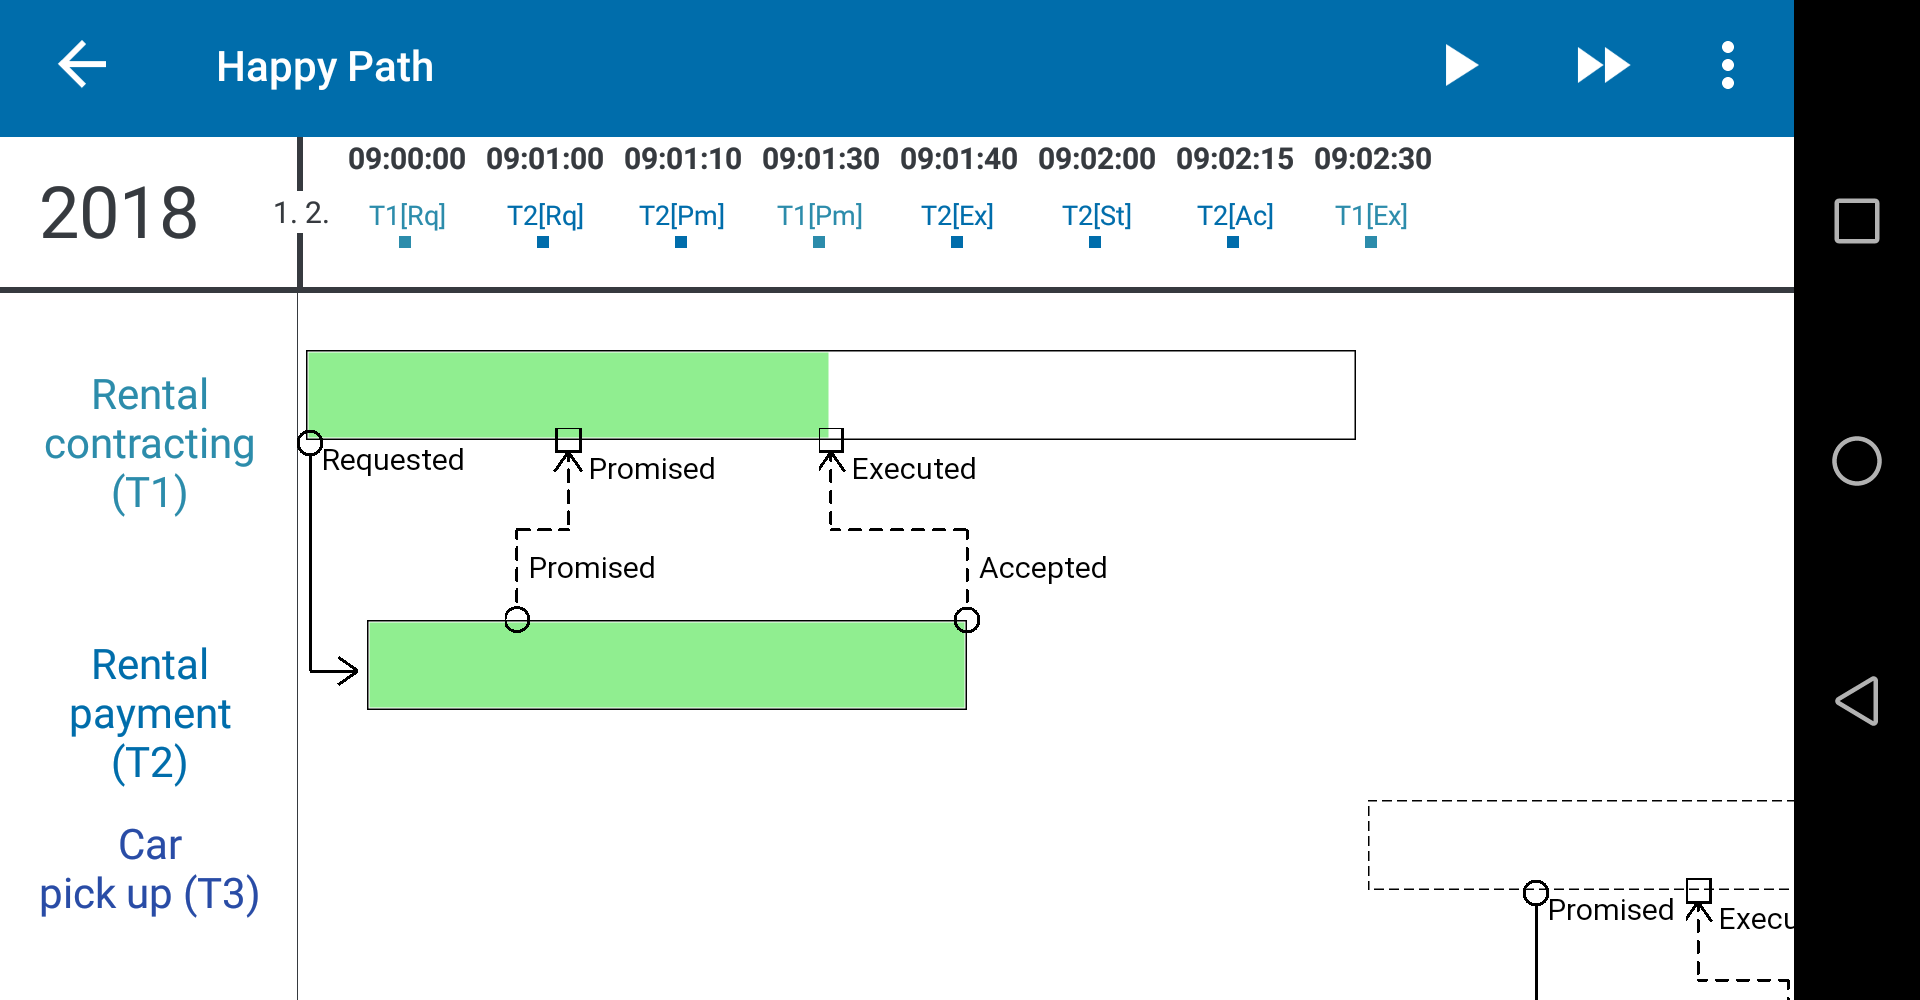
\includegraphics[width=12cm,keepaspectratio]{img/app-process-progress}
\caption{The process visualisation}
\label{fig:app-process-progress}
\end{figure}


